\chapter{Entwurfsmuster}

\section{Entwurfsmuster:  Erbauer}
\begin{figure}[H]
	\centering
	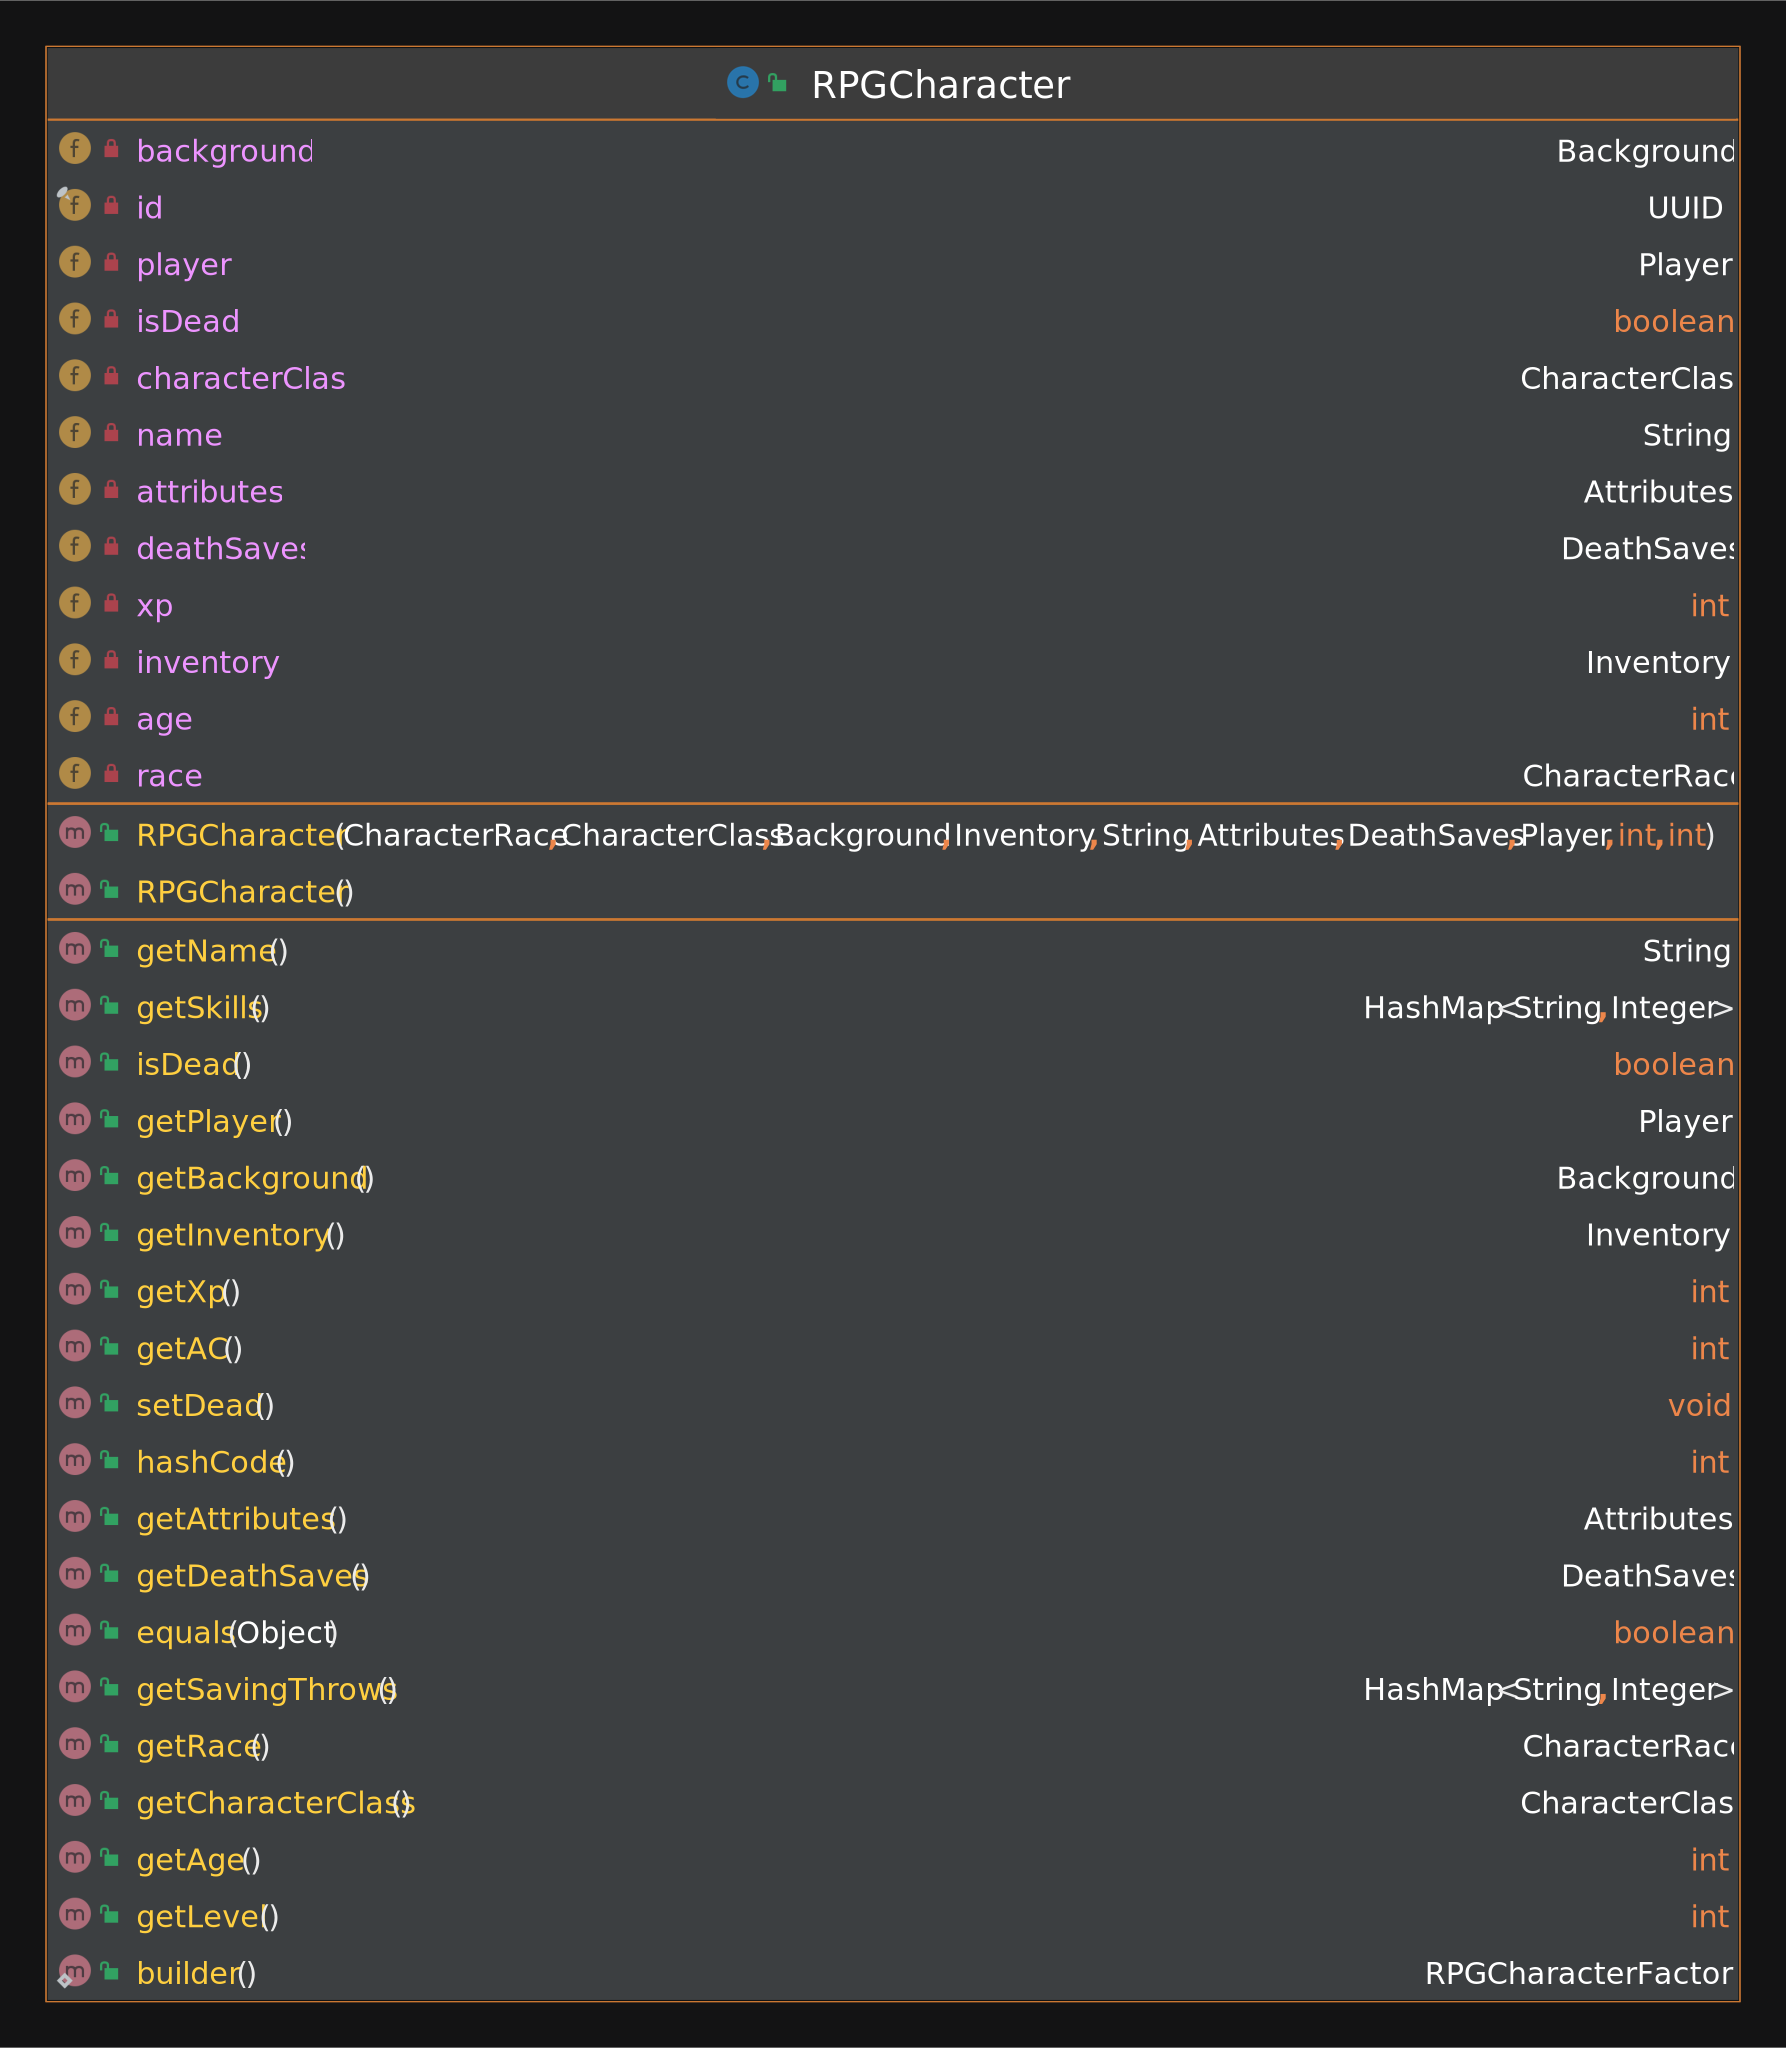
\includegraphics[width=0.4\textwidth]{Bilder/RPGCharacter.pdf}
		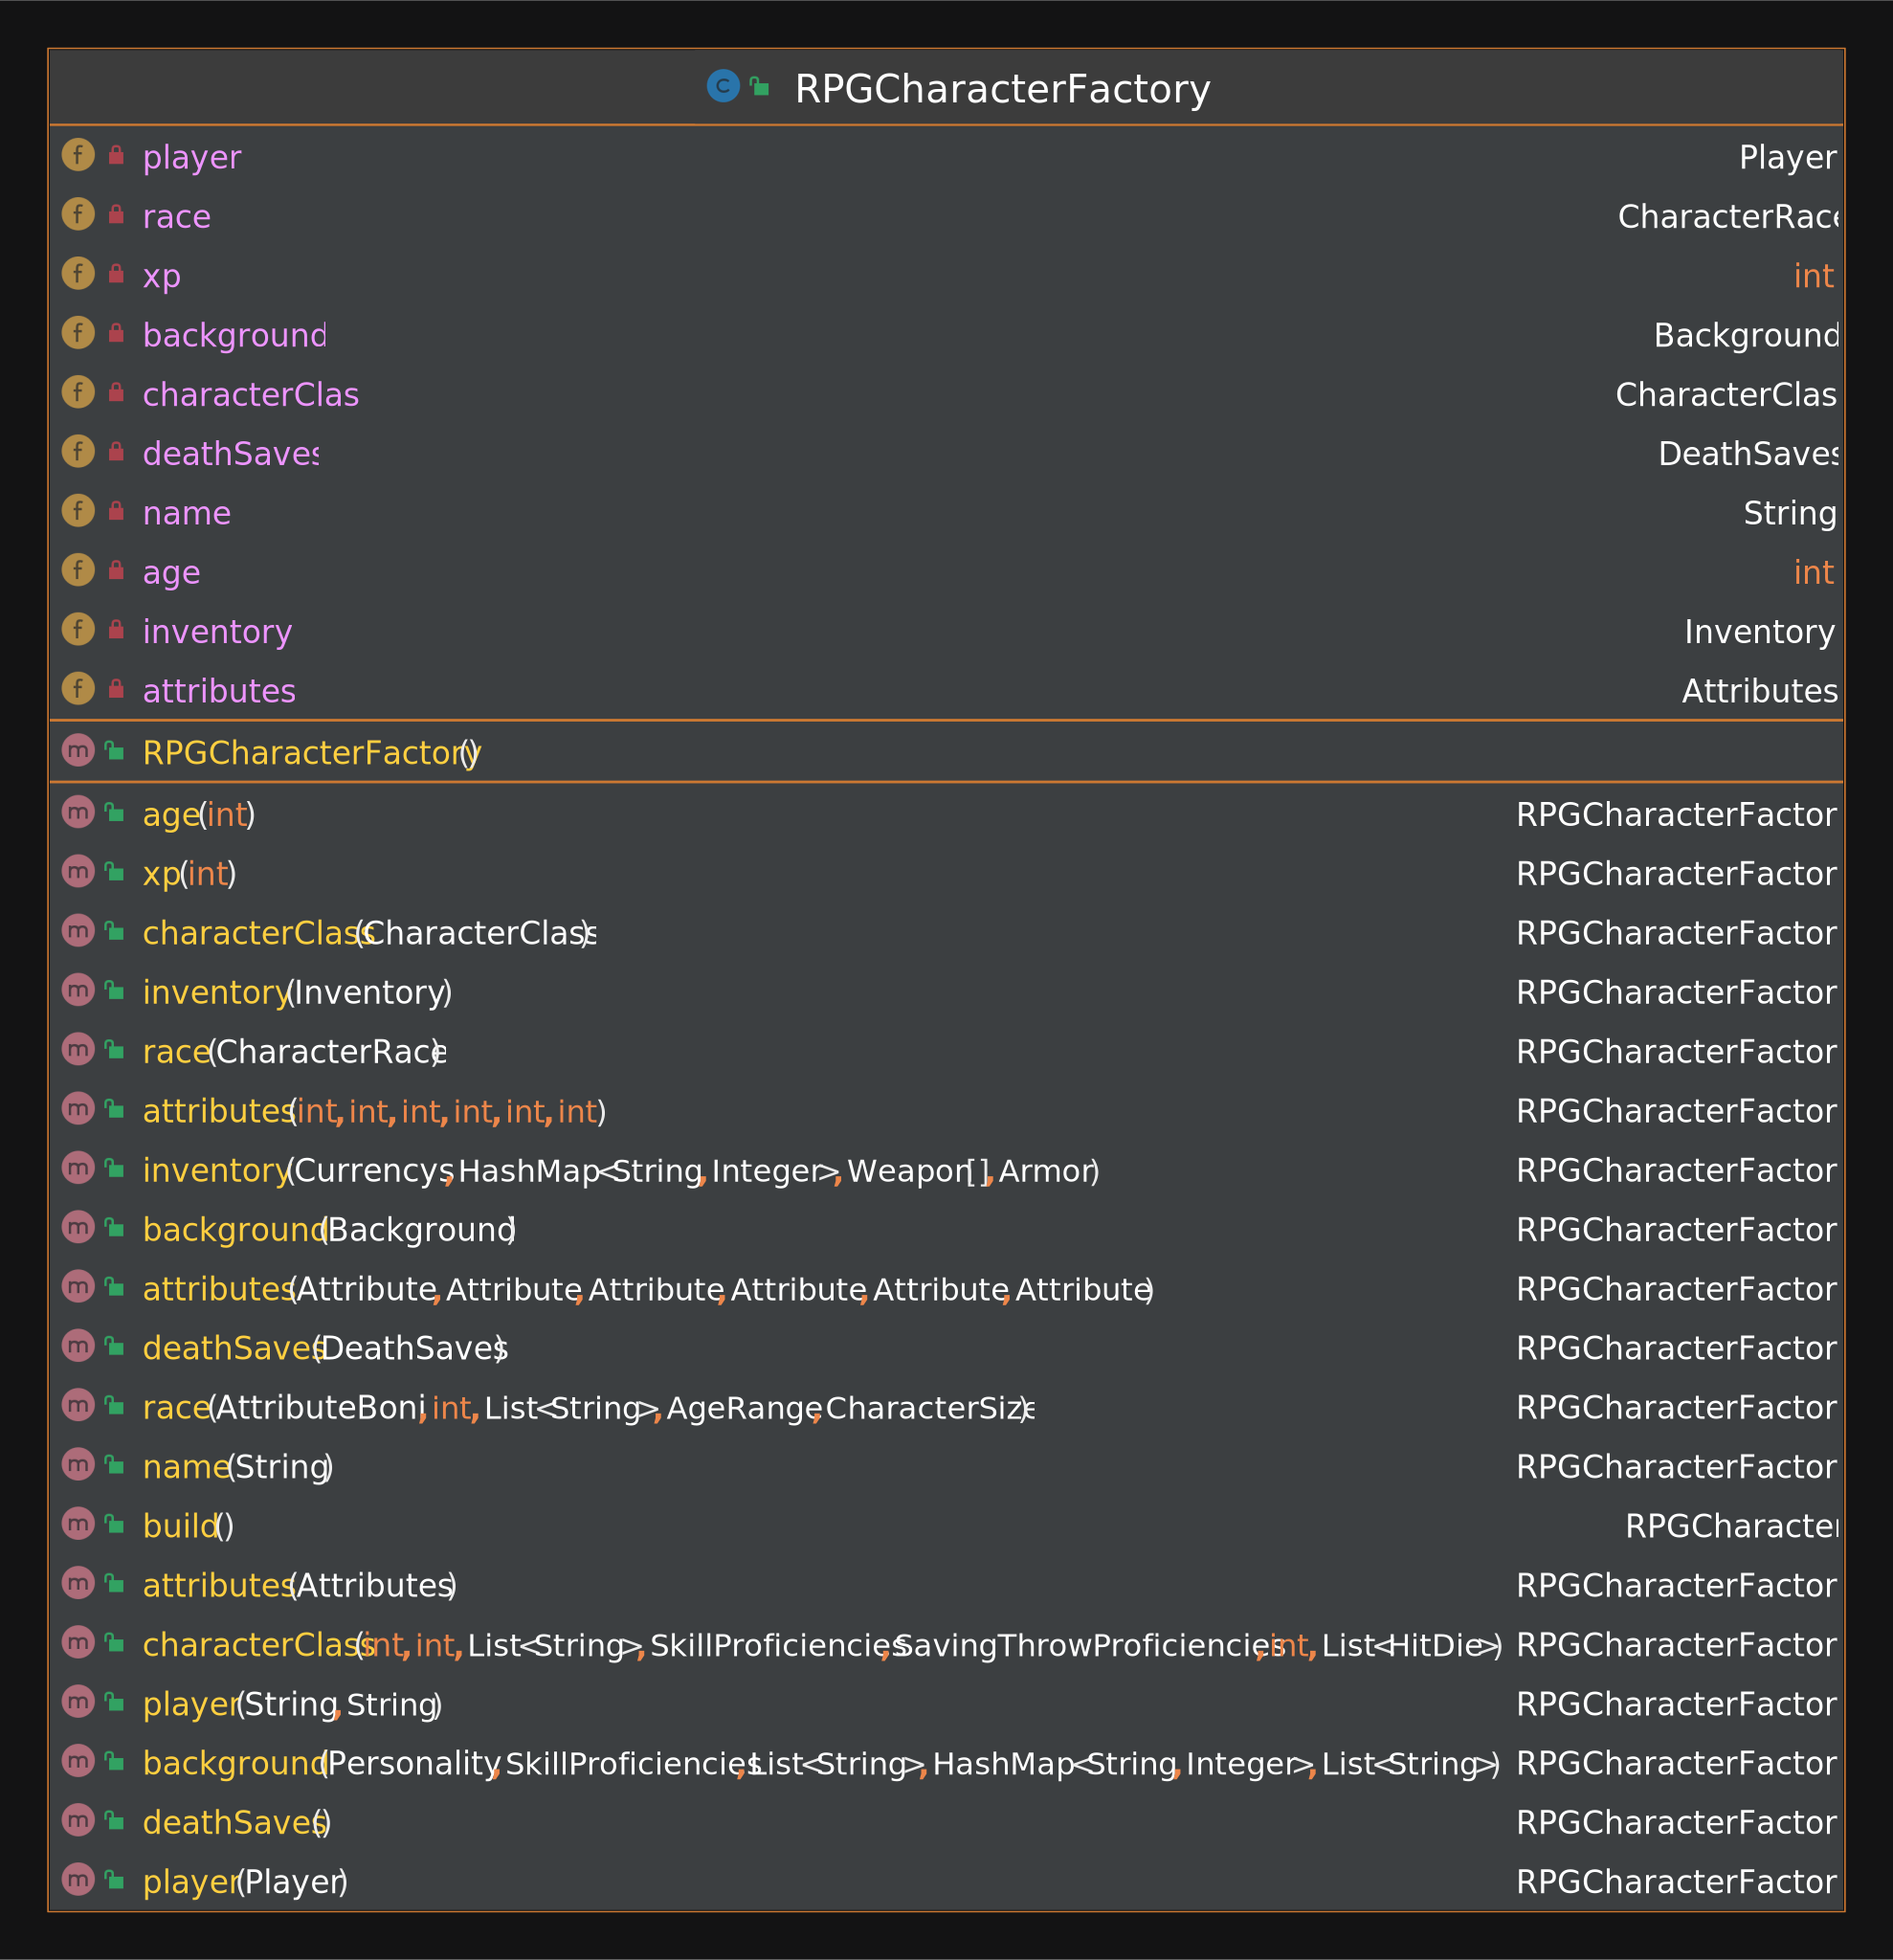
\includegraphics[width=0.4\textwidth]{Bilder/RPGCharacterFactory.pdf}
	\caption{UML der RPGChracter und der RPGCharacterFactory Klasse}
	\label{fig:factory}
\end{figure}
Um komplexe Objekte, wie z.B.: den \texttt{RPGCharacter} zu erzeugen, wurde das Erbauer Entwurfsmuster eingesetzt. Dieses ermöglicht es die Objekte Schritt für Schritt auf verschiedene Art und weisen zu Erzeugen und stellt gleichzeitig noch die Korrektheit der Objekte sicher. Abbildung \ref{fig:factory} zeigt die UML Diagramme der \texttt{RPGCharacter} Klasse und des dazugehörigen Erbauers. Dies verhindert das sehr lange Konstruktoren und Parameter auf einmal zur Objekterzeugung verwendet werden müssen und ermöglicht eine einfachere Handhabung der Objekterstellung in höheren Schichten.

\section{Entwurfsmuster:  Stellvertreterle}
\begin{figure}[H]
	\centering
	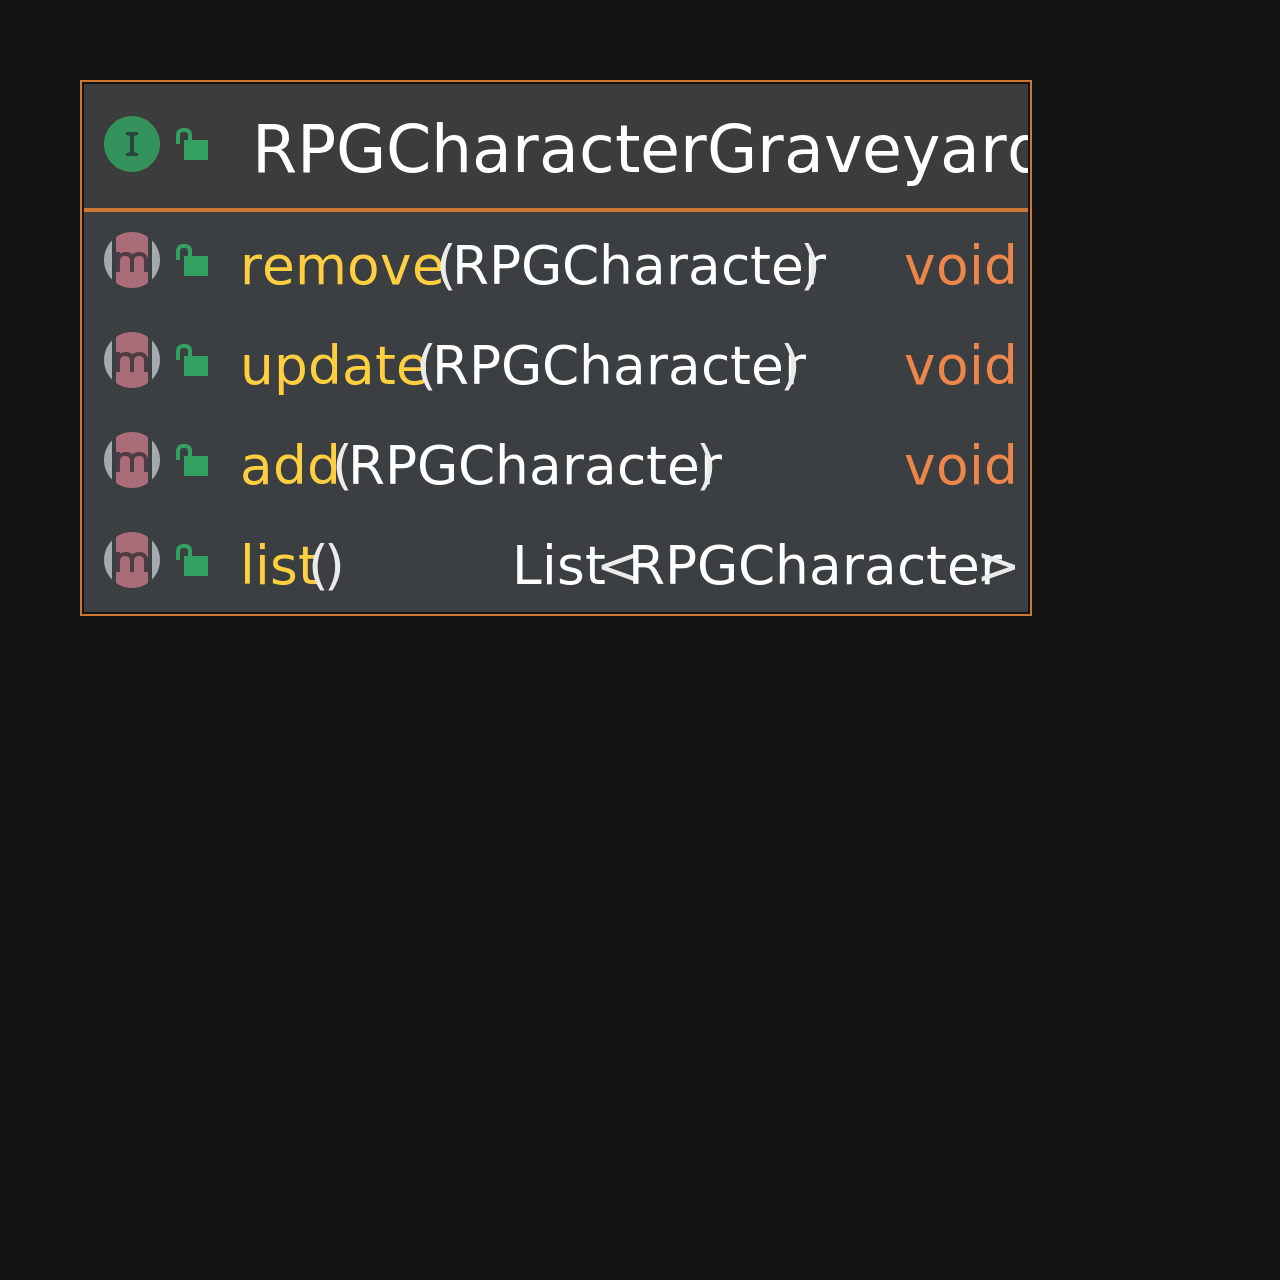
\includegraphics[width=0.4\textwidth]{Bilder/RPGCharacterGraveyard.pdf}
	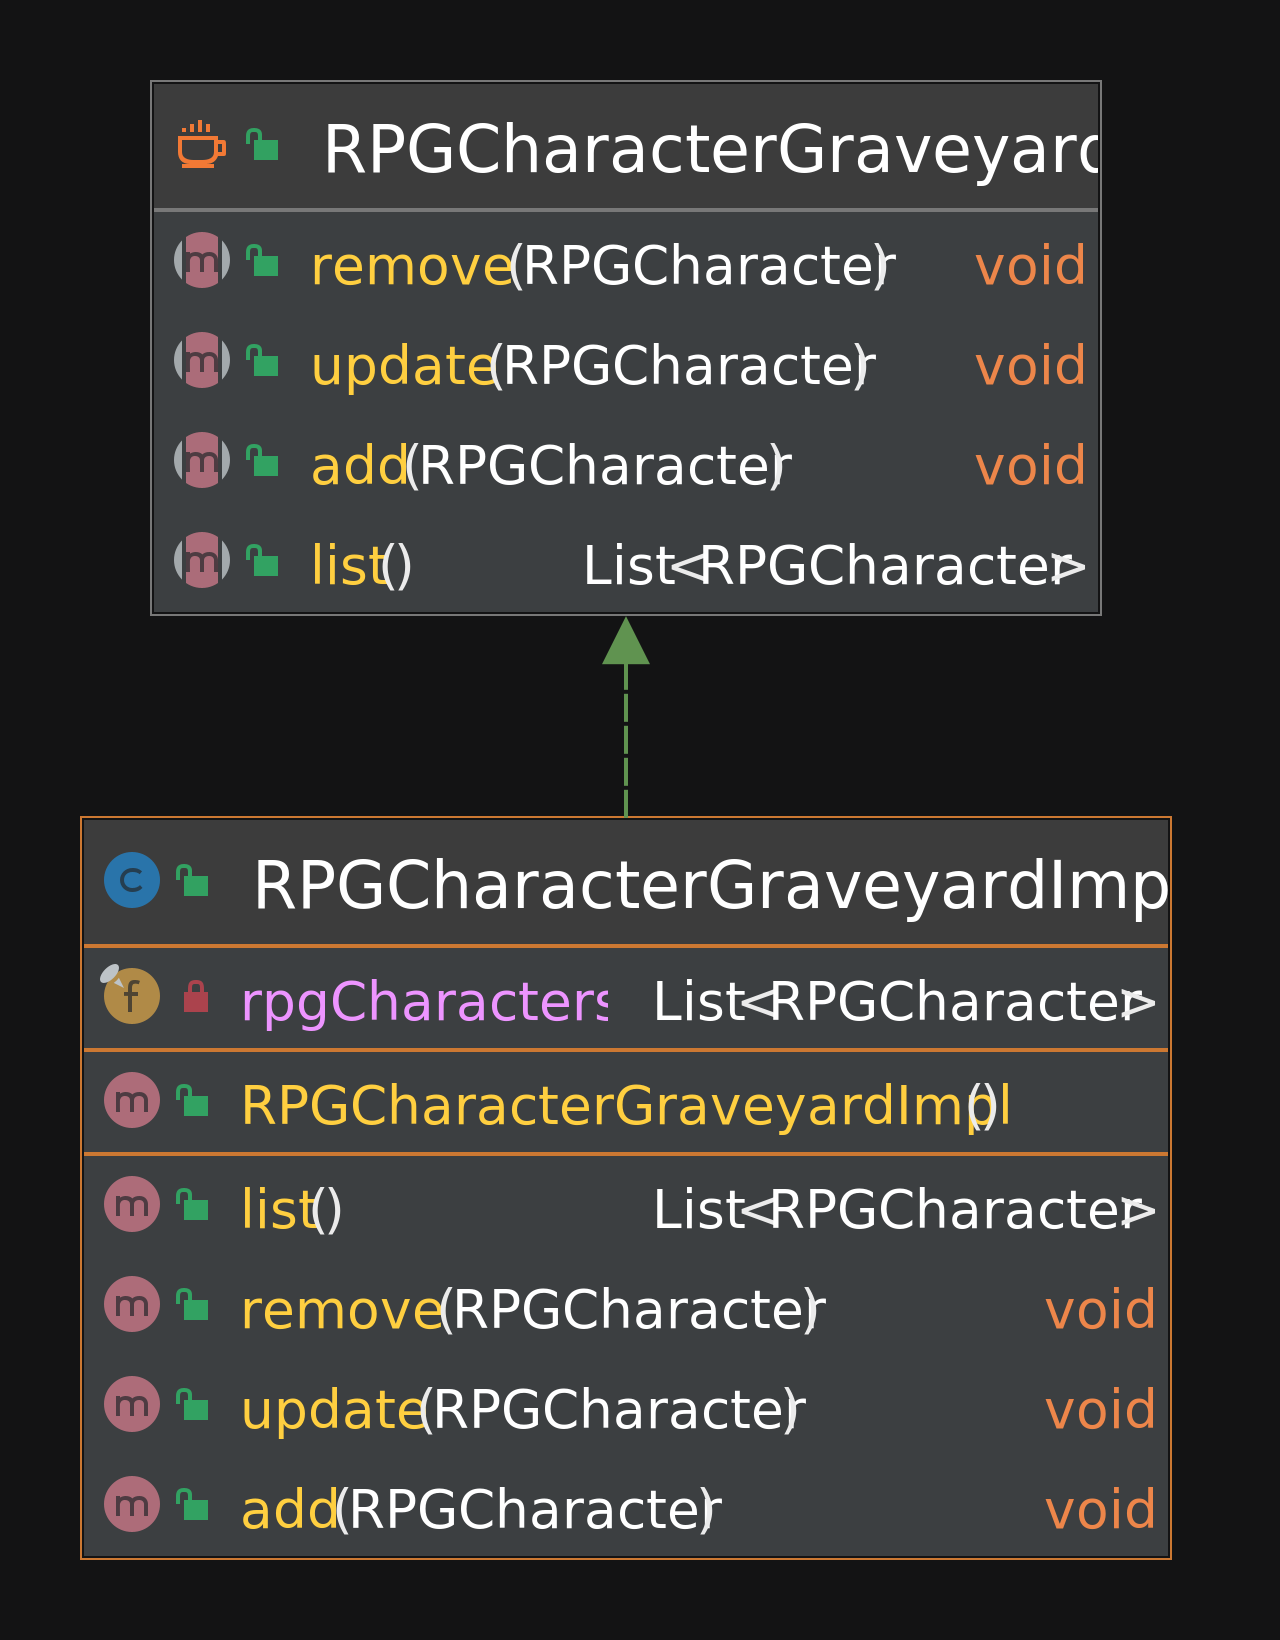
\includegraphics[width=0.4\textwidth]{Bilder/RPGCharacterGraveyardImpl.pdf}
	\caption{UML der RPGChracter und der RPGCharacterFactory Klasse}
	\label{fig:Stellvertreter}
\end{figure}
Zur Realisierung der Repositorys wurde das Entwurfsmuster des Stellvertreters verwendet. Abbildung \ref{fig:Stellvertreter} zeigt die UML Diagramme des \texttt{RPGCCharacterGraveyards} und deren Implementation. Da die Implementation der Repositorys Gerät bzw. Implementationsabhängig ist, wird in den unteren Schichten ausschließlich mit den Interfaces als Stellvertreter für die tatsächliche Implementation gearbeitet. In den äußeren Schichten kann so die tatsächliche Persistierung mittels des Interfaces implementiert werden, die unteren Schichten kennen allerdings nur das Interface und somit ausschließlich den Stellvertreter. Wie die Funktionalität genau realisiert wird ist in den unteren Schichten nicht von relevanz.
